\documentclass[conference]{IEEEtran}
\usepackage{graphicx}
\usepackage{amssymb}
\usepackage{algorithm}
\usepackage[noend]{distribalgo}
\usepackage{fixme}
\usepackage{xspace}
\usepackage{adjustbox}
\usepackage[usenames,dvipsnames,svgnames,table]{xcolor}
\usepackage[dvipsnames]{xcolor}

\newcommand{\ex}{$\mathcal{E}$}
\newcommand{\pp}{$\mathcal{P}$}
\newcommand{\ppm}{\mathcal{P}}
\newcommand{\oom}{\mathcal{O}}
\newcommand{\oo}{$\mathcal{O}$}
\newcommand{\cc}{$\mathcal{C}$}
\newcommand{\ccm}{\mathcal{C}}
\newcommand{\kk}{$\mathcal{K}$}
\newcommand{\vv}{$\mathcal{V}$}
\newcommand{\vvm}{\mathcal{V}}
\newcommand{\vvt}{$\mathcal{V}$}
\newcommand{\rr}{$\mathcal{R}$}
\newcommand{\rrm}{\mathcal{R}}
\newcommand{\sst}{$\mathcal{S}$}
\newcommand{\ssm}{\mathcal{S}}
\newcommand{\ip}{\mathcal{I}}
%
% S-SMR
\newcommand{\ssmr}{\mbox{S-SMR}\xspace}
\newcommand{\ssmrshort}{Scalable SMR}
\newcommand{\ssmrlong}{Scalable State Machine Replication}
%
% DS-SMR
\newcommand{\dssmr}{\mbox{DS-SMR}}
\newcommand{\dssmrshort}{Dynamic S-SMR}
\newcommand{\dssmrlong}{Dynamic Scalable State Machine Replication}
%
% The new DS-SMR system
\newcommand{\dynastar}{\mbox{DynaStar}\xspace}

% Eyrie and Chirper temporary name (double blind)
\newcommand{\libname}{Eyrie}   % rename to Eyrie   after paper is accepted
\newcommand{\appname}{Chirper} % rename to Chirper after paper is accepted
%
\newcommand{\rmcast}{r-mcast}
\newcommand{\rmdel}{r-deliver}
\newcommand{\amcast}{a-mcast}
\newcommand{\amdel}{a-deliver}
\newcommand{\parts}{partition}
\newcommand{\coloralgo}{Yellow}

\newcommand{\mynote}[3]{
   \fbox{\bfseries\sffamily\scriptsize#1}
   {\small$\blacktriangleright$\textsf{\emph{\color{#3}{#2}}}$\blacktriangleleft$}}
\newcommand{\fp}[1]{\mynote{Fernando}{#1}{Red}}
\newcommand{\eb}[1]{\mynote{Eduardo}{#1}{Green}}
\newcommand{\ef}[1]{\mynote{Enrique}{#1}{Blue}}

\newcommand{\red}[1]{\textit{\textcolor{red}{#1}}}

\begin{document}

\title{\dynastar: Quasi-Optimum Dynamic Partitioning for Scalable State Machine Replication}
%\title{\dynastar: Near-Optimum Dynamic Partitioning for Scalable State Machine Replication}
%\title{Locality-aware scalable state machine replication}
%\title{Locality-aware partitioned state machine replication: Designing scalable systems that scale}
%\title{On the power of locality: Designing partitioned systems that fulfill their promises}

%\author{\IEEEauthorblockN{}
%\IEEEauthorblockA{}
%\and
%\IEEEauthorblockN{}
%\IEEEauthorblockA{}
%\and
%\IEEEauthorblockN{}
%\IEEEauthorblockA{}}

\maketitle
\thispagestyle{plain}
\pagestyle{plain}

\begin{abstract}
%Borrow from SSMR paper

%State machine replication (SMR) is a well-known technique to provide high availability and strong consistency (i.e., linearizability) to online services.
%In SMR, client commands are executed in the same order on all server replicas: after executing each client command, every replica will reach the same state. 
%%
%One problem is that the original SMR model lacks scalability, as every replica executes all commands.
%Because of that, adding replicas does not increase the maximum system throughput.
%%
%Scalable SMR (\ssmr) addresses this problem by partitioning the service state, allowing client commands to be executed only by some replicas, while still ensuring linearizability.
%By doing this, \ssmr\ scales linearly with the number of partitions for workloads where each command accesses a single partition.
%%
%However, \ssmr\ may quickly become saturated when executing multi-partition commands,
%as they require communication between partitions.
%Dynamic S-SMR (\dssmr) solves this problem by repartitioning the state dynamically, based on the workload.
%When a command needs variables from different partitions, those variables are first moved to the same partition.
%Then, the command is executed as a single-partition command.
%As a result, variables that are usually accessed together will tend to stay in the same partition, significantly improving scalability.
%We evaluate the performance of \dssmr\ with a scalable social network application.

State machine replication (SMR) is a well-known technique that guarantees strong consistency (i.e., linearizability) to online services.
In SMR, client commands are executed in the same order on all server replicas: after executing each command, every replica reaches the same state.
However, SMR lacks scalability: every replica executes all commands, so adding servers does not increase the maximum throughput.
Scalable SMR (\ssmr) addresses this problem by partitioning the service state, allowing commands to execute only in some replicas, providing scalability while still ensuring linearizability.
One problem is that ssmr quickly saturates when executing multi-partition commands,
as partitions must communicate.
\dssmrshort\ (\dssmr) solves this issue by repartitioning the state dynamically, based on the workload.
Variables that are usually accessed together are moved to the same partition, which significantly improves scalability.
We evaluate the performance of \dssmr\ with a scalable social network application.

\end{abstract}
%!TEX root =  main.tex
\section{Introduction}


\begin{figure*}[ht!]
  \centering
  \begin{subfigure}[b]{0.45\textwidth}
    \centering
    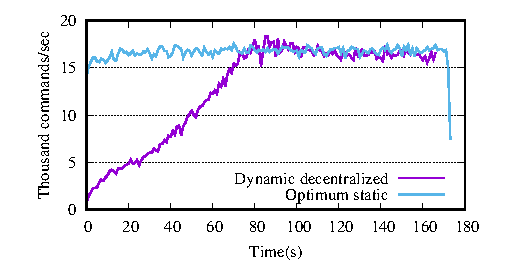
\includegraphics[width=0.95\columnwidth]{figures/motivation-tp-strong-locality}    
    \caption{Throughput with strong locality.}
  \end{subfigure}
  \begin{subfigure}[b]{0.45\textwidth}
    \centering
    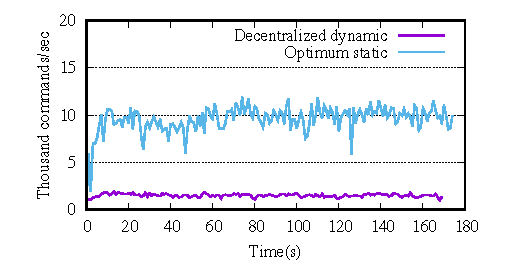
\includegraphics[width=0.95\columnwidth]{figures/motivation-tp-weak-locality}
    \caption{Throughput with weak locality}
  \end{subfigure} \\
  \begin{subfigure}[b]{0.45\textwidth}
    \centering
    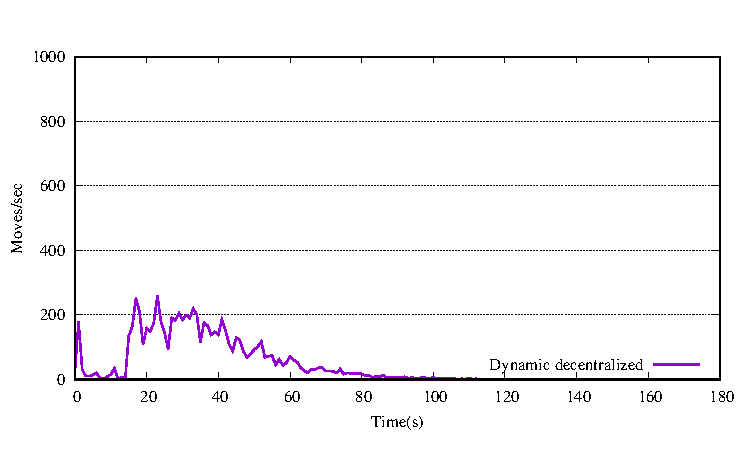
\includegraphics[width=0.95\columnwidth]{figures/motivation-moves-strong-locality}
    \caption{Number of move commands with strong locality.}
  \end{subfigure}
  \begin{subfigure}[b]{0.45\textwidth}
    \centering
    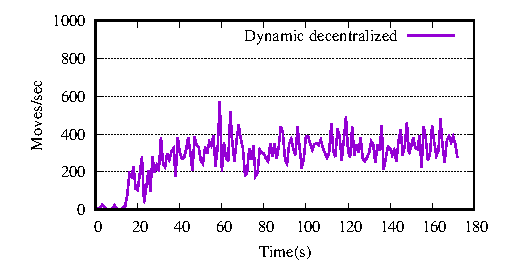
\includegraphics[width=0.95\columnwidth]{figures/motivation-moves-weak-locality}
    \caption{Number of move commands with weak locality}
  \end{subfigure} 
\end{figure*}




State machine replication (SMR) is a fundamental technique for
building fault tolerant systems and services. With SMR, state is
replicated on a set of servers, and each replica deterministically
executes the same sequence of client commands in order to maintain
consistency. Unfortunately, classic state machine replication does not
scale, since each replica must execute every command. In order to
improve the scalability of SMR, several systems have investigated the
use of state partitioning~\cite{facebookTAO, sciascia2012sdur,
  Aguilera:2007}.

In principle, increasing the number of partitions should result in
increased system performance. However, if executing a command
requires that the system access multiple partitions, then performance
can actually decrease, due to overhead from ordering commands across partitions to
ensure strong consistency. Moreover, if data is not distributed
carefully, then load imbalances can nullify the benefits of
partitioning.  Thus, an ideal partitioning scheme is one that would
both (i) minimize multiple partition commands, and (ii) provide load
balancing among the partitions. We refer to workloads that can be
partitioned in a way that satisfies these two properties as exhibiting
\emph{strong locality}.
\ef{i) and ii) don't imply our definition of strong locality}

Broadly speaking, there are two classes of techniques for
partitioning: \emph{static} and \emph{dynamic}.
Figure~\ref{fig:motivation} shows the result of a motivating experiment
that highlights the shortcomings of both of these approaches. In
the experiment, we show the throughput and number of state moves
over time with two different workloads; one with strong locality
and one with weak locality. For brevity, we postpone the details
of the experimental setup until Section~\ref{sec:experiments}.

Static schemes choose an immutable assignment of objects to partitions in
advance.  A prominent example of a
static scheme is S-SMR~\cite{bezerra2014ssmr}. One problem with static schemes is
that they cannot adapt as workloads change over time (e.g., in social
networks users join and leave the system, connections are created and
removed). One could imagine a static scheme that re-partitioned the
data based on every change in workload, but such a scheme would be
impossible to implement, since it would require a priori knowledge of
the workload. Figure~\ref{fig:motivation} shows the theoretical
optimal throughput one could achieve with a ``perfect'' static scheme.


Dynamic schemes are designed to address the problem with static
schemes.  Dynamic schemes assume no prior knowledge of the workload,
and move data to partitions on-demand in order to avoid
multi-partition commands. A prominent example of a dynamic scheme is
DS-SMR~\cite{hoang2016}. Unfortunately, existing dynamic schemes assume
workloads with strong locality. As Figure~\ref{fig:motivation} shows,
for workloads with weak-locality, DS-SMR suffers from instability due
to constantly moving data from one partition to another.


In this paper, we introduce \dynastar, a new approach to the state
partitioning problem designed to address these challenges.  \dynastar
is \emph{dynamic}. It does not require any a priori knowledge about
the workload, and it adapts to workload changes on-the-fly. However,
it is able to achieve throughputs comparable to the unrealizable
perfect static scheme. The key idea behind \dynastar is that it
minimizes the number of state relocations by monitoring the workload,
and re-computing an optimal partitioning on demand using a static
partitioner, we chose to use METIS partitioning algorithm~\cite{Abou-Rjeili:2006}
as an example of a static partitioner.
%ef.: Changed so we allow plug-and-play partitioners


With \dynastar, a location oracle maintains two data structures: (i) a
mapping of objects to partitions, and (ii) a \emph{workload graph}
with objects as vertices and edges as commands that access the
objects.  When a client submits a command, it must first contact the
location oracle to discover the partitions on which the objects are
stored.  If the command accesses objects in multiple partitions, the
oracle issues a move command to the partitions, re-locating objects to
a single partition. Of course, when re-locating an object, the oracle
is faced with a choice of which partition to use as a destination.
\dynastar chooses the optimal partition for relocation (i.e., one that
would minimize the number of state relocations) by partitioning the
workload graph using the METIS partitioner.




We have fully implemented \dynastar and compared its performance to
the dynamic partitioning protocol proposed by Long et
al.~\cite{hoang2016} and to the optimized static partitioning scheme.
Our prototype can handle workload graphs with half a million variables
and tens of millions of connections.  In workloads that present strong
locality, all three protocols eventually delivered comparable
performance, although \dynastar converged more quickly than the
decentralized scheme.  In workloads with weak locality, however,
\dynastar \emph{outperformed both} schemes.  The reason for the
surprisingly high performance of \dynastar compared to the optimized
static partitioning scheme is that \textbf{we need to explain this!!!
  :-)} \ef{If the cost of migrating the object outperforms the cost of signaling partitions,
  why performance get similar when we have more partitions?} \lle{this is true in the case of 
	weak locality, but not true if workload could be perfectly partitioned, since there is 
	exchange of signal nor data. I updated the graph with proper numbers}

The paper makes the following contributions:
\begin{itemize}
\item It introduces \dynastar and discusses its implementation. 
\item It evaluates different partitioning schemes for state machine replication under a variety of conditions.
\item It describes \appname{} to demonstrate how \libname{} can be used to implement a scalable social network service.
\item It presents a detailed experimental evaluation of \dynastar including real social network graphs with half a million users and 14 million edges.
\end{itemize}

The rest of the paper is structured as follows.
Section~\ref{sec:sysmodel} describes our system model.
Section~\ref{sec:background} reviews existing scalable state machine replication approaches.
Section~\ref{sec:dssmr} introduces \dssmr{}; we explain the technique in detail and argue about its correctness.
Section~\ref{sec:implementation} details the implementation of \libname\ and \appname{}.
Section~\ref{sec:experiments} reports on the results of our experiments with \dssmr{}.
Section~\ref{sec:rw} surveys related work and
Section~\ref{sec:conclusion} concludes the paper.




%% %% Because single-partition commands are much more efficient than
%% %% multi-partition commands (i.e., in some cases by a factor of more than
%% %% 10x), the performance of a distributed storage system is particularly sensitive to the way
%% %% the service state is partitioned.


%% \subsection{State Machine Replication}

%% State machine replication (SMR) is a well-established technique to
%% develop highly available services (e.g.,
%% \cite{Shvachko:2003,Ghemawat:2003,Burrows:2006,MacCormick:2004}).  In
%% essence, the idea is that replicas deterministically execute the same
%% sequence of client commands in the same order and in doing so traverse
%% the same sequence of states and produce the same results.  State
%% machine replication provides configurable fault tolerance in the sense
%% that the system can be set to tolerate any number of faulty replicas.
%% Increasing the number of replicas, however, will not scale performance
%% since each replica must execute every command.  Unfortunately,
%% increasing the number of replicas will not scale performance since
%% each replica must execute every command.

%% S-SMR relies on an atomic multicast primitive to consistently order
%% commands within and across partitions.  Commands that access objects
%% located in a single partition (i.e., single-partition commands) are
%% multicast to the concerned partition and executed like in classical
%% SMR.  Commands that access objects located in multiple partitions
%% (i.e., multi-partition commands) are multicast to all involved
%% partitions.  To prevent command interleaves that violate strong
%% consistency, partitions coordinate during the execution of
%% multi-partition commands.



%% \subsection{Motivating Example}

\clearpage
%!TEX root =  main.tex
\section{System model and definitions}
\label{sec:sysmodel}

In this section, we present the system model, and define our
correctness criterion (i.e., linearizability). Additionally, because
\dynastar relies on two variations of a multicast primitive for
communication, we discuss them below. When the protocol requires that
commands are consistently ordered across partitions, \dynastar uses
atomic multicast. Otherwise, it uses a reliable multicast, which has
less overhead.


%\red{How do we use reliable multicast, as opposed to atomic?}
%\red{Do we need this primitive? Or is it just inherited from the artifact?}
%\lle{Partitions (and oracle) in \dynastar use reliable multicast to exchange
% objects and signals }
%% S-SMR relies on an atomic multicast primitive to consistently order
%% commands within and across partitions.  Commands that access objects
%% located in a single partition (i.e., single-partition commands) are
%% multicast to the concerned partition and executed like in classical
%% SMR.  Commands that access objects located in multiple partitions
%% (i.e., multi-partition commands) are multicast to all involved
%% partitions.  To prevent command interleaves that violate strong
%% consistency, partitions coordinate during the execution of
%% multi-partition commands.




\subsection{Processes and communication}

We consider a distributed system consisting of an unbounded set of
client processes $\ccm = \{c_1, c_2, ...\}$ and a bounded set of
server processes (replicas) $\ssm = \{s_1, ..., s_n\}$.  Set $\ssm$ is
divided into disjoint groups of servers $\ssm_0, ..., \ssm_k$.
Processes are either \emph{correct}, if they never fail, or
\emph{faulty}, otherwise.  In either case, processes do not experience
arbitrary behavior (i.e., no Byzantine failures).

Processes communicate by message passing, using either one-to-one or
one-to-many communication.  The system is asynchronous: there is no
bound on message delay or on relative process speed.  One-to-one
communication uses primitives $send(p,m)$ and $receive(m)$, where $m$
is a message and $p$ is the process $m$ is addressed to.  If sender
and receiver are correct, then every message sent is eventually
received.
%
One-to-many communication relies on reliable multicast and atomic
multicast,\footnote{Solving atomic multicast requires additional
  assumptions~\cite{CT96,FLP85}. In the following, we simply assume
  the existence of an atomic multicast oracle.}  defined in
sections~\ref{sec:rmcast} and \ref{sec:amcast}, respectively.


\subsection{Correctness criterion}
\label{sec:correctcrit}

Our consistency criterion is linearizability.  A system is
\emph{linearizable} if there is a way to reorder the client commands
in a sequence that (i)~respects the semantics of the commands, as
defined in their sequential specifications, and (ii)~respects the
real-time precedence of commands~\cite{Attiya04}.


\subsection{Reliable multicast}
\label{sec:rmcast}

To reliably multicast a message $m$ to a set of groups $\gamma$,
processes use primitive \rmcast$(\gamma, m)$.  Message $m$ is
delivered at the destinations with \rmdel$(m)$.  Reliable multicast
has the following properties:

\begin{itemize}

    \item[--] If a correct process \rmcast{}s $m$, then every correct
      process in $\gamma$ \rmdel{}s $m$ \emph{(validity)}.
    
    \item[--] If a correct process \rmdel{}s $m$, then every correct
      process in $\gamma$ \rmdel{}s $m$ \emph{(agreement)}.
    
    \item[--] For any message $m$, every process $p$ in $\gamma$
      \rmdel{}s $m$ at most once, and only if some process has
      \rmcast{} $m$ to $\gamma$ previously \emph{(integrity)}.
    
\end{itemize}

\subsection{Atomic multicast}
\label{sec:amcast}

To atomically multicast a message $m$ to a set of groups $\gamma$,
processes use primitive \amcast$(\gamma, m)$.  Message $m$ is
delivered at the destinations with \amdel$(m)$.  We define delivery
order $<$ as follows: $m < m'$ iff there exists a process that
delivers $m$ before $m'$.

Atomic multicast ensures the following properties:

\begin{itemize}
    
    \item[--] If a correct process \amcast{}s $m$, every correct
      process in a group in $\gamma$ \amdel{}s $m$ \emph{(validity)}.
    
    \item[--] If a process \amdel{}s $m$, then every correct process
      in a group in $\gamma$ \amdel{}s $m$ \emph{(uniform agreement)}.
    
    \item[--] For any message $m$, every process \amdel{}s $m$ at most
      once, and only if some process has \amcast{} $m$ previously
      \emph{(integrity)}.
    
    \item[--] The delivery order is acyclic \emph{(atomic order)}.

    \item[--] For any messages $m$ and $m'$ and any processes $p$ and
      $q$ such that $p \in g$, $q \in h$ and $\{ g, h \} \subseteq
      \gamma$, if $p$ delivers $m$ and $q$ delivers $m'$, then either
      $p$ delivers $m'$ before $m$ or $q$ delivers $m$ before $m'$
      \emph{(prefix order)}.
    
\end{itemize}

Atomic broadcast is a special case of atomic multicast in which there
is a single group of processes.


%!TEX root =  main.tex
\section{Background}
\label{sec:background}

\dynastar builds on state machine replication and scalable state machine replication.
In this section, we recall these techniques and the dynamic partitioning scheme proposed by Long et al.~\cite{hoang2016}.

\subsection{State Machine Replication (SMR)}
\label{sec:smr}

State machine replication is a fundamental approach to implementing fault-tolerant services by replicating servers, and coordinating the execution of client commands at server replicas~\cite{Lam78,Sch90}. 
SMR ensures linearizability~\cite{Attiya04} by coordinating the execution of commands in the different replicas: 
Every replica has a full copy of the service state, identified by a set of state variables $\vvm = \{v_1, ..., v_m\}$.
Replicas execute commands submitted by the clients in the same order. 
A command is a sequence of deterministic operations that can read and modify the state.
%program consisting of a sequence of operations, which can be of three types: $read(v)$, $write(v, val)$, or a deterministic computation.

By starting in the same initial state and executing the same sequence of deterministic commands, servers make the same state changes and produce the same reply for each command. To guarantee that servers deliver the same sequence of commands, SMR can be implemented with atomic broadcast: commands are atomically broadcast to all servers, and all correct servers deliver and execute the same sequence of commands \cite{BJ87b,DSU04}.

Despite its simple execution model, classical SMR does not scale: adding resources (e.g., replicas) will not translate into sustainable improvements in throughput. 
%This happens for two reasons. 
%First, the underlying communication protocol needed to ensure ordered message delivery may itself not scale (i.e., a communication bottleneck). 
%Second, every command must be executed sequentially by each replica (i.e., an execution bottleneck).
%
Several approaches have been proposed to address SMR's scalability limitations. 
In the following, we review two state machine replication approaches that partition the service's state and replicate each partition (e.g., \cite{Glendenning:2011kj,Marandi:2011dj,hoang2016}).
%Scalable State Machine Replication (\ssmr), an approach that partitions the service's state and replicates each partition (e.g., \cite{Glendenning:2011kj,Marandi:2011dj,hoang2016}).


\subsection{Scalable State Machine Replication (S-SMR)}
%\subsection{Scalable replication with static state partitioning}
%\subsection{S-SMR with static partitioning}
\label{sec:ssmr}

%
%To cope with communication overhead, some proposals have suggested to spread the load of ordering commands among multiple processes (e.g., \cite{Moraru:2013gw,Mencius,Marandi:2012hb}), as opposed to dedicating a single process to determine the order of commands (e.g., \cite{Lamport:1998ea}).%\fxnote[draft]{remove inapplicable reference}
%
%Two directions of research have been suggested to overcome execution bottlenecks. One approach (scaling up) is to take advantage of multiple cores to execute commands concurrently without sacrificing consistency \cite{Kapritsos:2012um,Marandi:2014bj,Kotla:2004ep,Guo:2014jp}.
%% Remove candidate: END
%Another approach (scaling out) is to partition the service's state and replicate each partition (e.g., \cite{Glendenning:2011kj,Marandi:2011dj}). 
%In the next few sections, we review Scalable State Machine Replication (\ssmr) and its dynamic-partitioning variant \dssmr, both proposals related to scaling out the state.
%
In S-SMR~\cite{bezerra2014ssmr}, the service state \vvt\ is composed of $k$ partitions, $\ppm_1, ..., \ppm_k$, where each partition $\ppm_i$ is statically assigned to server group $\ssm_i$. 
For brevity, we say that server $s$ belongs to $\ppm_i$ meaning that $s \in \ssm_i$, and say ``multicast to $\ppm_i$" meaning ``multicast to server group $\ssm_i$".
S-SMR relies on an \emph{oracle}, which tells which partitions are accessed by each command.
%\footnote{The oracle returns a set with the partitions accessed by the command, but this set does not need to be minimal; it may contain all partitions in the worst case, when the partitions accessed by the command cannot be determined before the command is executed.}

To execute a command, a client multicasts the command to the appropriate partitions, as determined by the oracle.
Commands that access a single partition are executed as in classical SMR: replicas of the concerned partition agree on the execution order and each replica executes the command independently.
In the case of a multi-partition command, replicas of the involved partitions deliver the command and then may need to exchange state, since some partitions may not have all the values read in the command.
This mechanism allows commands to execute seamlessly despite the partitioned state.

%\begin{algorithm}[t!]
\small

\begin{distribalgo}[1]

\vspace{1mm}

\INDENT{\emph{Initialization:}}
    \STATE $\forall C \in $ \kk $ : rcvd\_signals(C) \leftarrow \emptyset$
    \STATE $\forall C \in $ \kk $ : rcvd\_variables(C) \leftarrow \emptyset$
\ENDINDENT

\vspace{1.25mm}
\INDENT{\emph{Command $C$ is submitted by a client as follows:}}
    \STATE $C.dests \leftarrow oracle(C)$ \label{algline:oracle} 
	\STATE \amcast$(C.dests, C)$ \label{algline:climcast}
	\STATE wait for reply
\ENDINDENT

\vspace{1.25mm}
\INDENT{\emph{Server $s$ of partition \pp\ executes command $C$ as follows:}}
	\INDENT{\textbf{when} \amdel$(C)$}
	    \STATE $others \leftarrow C.dests \setminus \{\ppm{}\}$
	    \STATE \rmcast$(others, signal(C))$ \label{algline:mcastsignals}
		\FOR{each operation $op$ in $C$}
			\IF{$op$ is $read(v)$}
			    \IF{$v \in \ppm$}
			        \STATE \rmcast$(others, \langle v, C.id \rangle)$ \label{algline:multicastv}
			    \ELSE
			        \STATE \textbf{wait until} $v \in rcvd\_variables(C)$ \label{algline:waitvariable}
			        \STATE update $v$ with the value in $rcvd\_variables(C)$
			    \ENDIF
			\ENDIF
			\STATE execute $op$ \label{algline:executeopck}
		\ENDFOR
		\STATE \textbf{wait until} $rcvd\_signals(C) = others$ \label{algline:waitsignals}
		\STATE send reply to client \label{algline:sendreply}
	\ENDINDENT
	
	\vspace{1.25mm}
	\INDENT{\textbf{when} \rmdel$(signal(C))$ from partition $\ppm'$}
	    \STATE $rcvd\_signals(C) \leftarrow rcvd\_signals(C) \cup \{\ppm'\}$
	\ENDINDENT

	\vspace{1.25mm}
	\INDENT{\textbf{when} \rmdel$(\langle v, C.id \rangle)$}
	    \STATE $rcvd\_variables(C) \leftarrow rcvd\_variables(C) \cup \{v\}$
	\ENDINDENT
			
\ENDINDENT

\vspace{1.7mm}

\textbf{Algorithm variables:}

\vspace{1.25mm}

\kk: the set of all possible commands

\vspace{1mm}

$C.id$: unique identifier of command $C$

\vspace{1mm}

$oracle(C)$: function that returns a superset of the partitions accessed by $C$

\vspace{1mm}

$C.dests$: set of partitions to which $C$ is multicast

\vspace{1mm}

$others$: set of all partitions, other than \pp{}, where $C$ is executed.

\vspace{1mm}

$signal(C)$: signal exchanged to ensure linearizability

\vspace{1mm}

$rcvd\_signals(C)$: set of all partitions that already signaled \pp\ regarding $C$

\vspace{1mm}

$rcvd\_variables(C)$: set of all variables received from other partitions in order to execute $C$

\caption{Scalable State Machine Replication (\ssmr)}
\label{alg:ssmr}
\end{distribalgo}
\end{algorithm}

%\begin{figure*}
%\begin{minipage}[b]{1\linewidth} % A minipage that covers the whole width of the page
%\centering
%      \includegraphics[width=1.0\linewidth]{figures/move_case_1}
%\end{minipage}
%\caption{Consulting the oracle and issuing a command are done in multiple calls to \amcast{}. White boxes represent actions of the client proxy.}
%\label{fig:move_case_1}
%\end{figure*}

%Algorithm~\ref{alg:ssmr} shows precisely how S-SMR operates. 
In more detail, when a server $s$ of partition $\ppm$, while executing a command $C$, reaches a $read(v)$ operation, there are two possibilities:
either $v$ belongs to the local partition $\ppm$,
or it is part of a remote partition $\ppm'$. 
If $v$ is local, $s$ will retrieve its value and send it to the servers of other partitions concerned by $C$;
if $v$ is remote, $s$ will wait until its value is received from a server of $\ppm'$. 
A $write(v, val)$ operation does not depend on the previous value of $v$, not requiring communication between partitions, even if $v$ is not assigned to the partition of the server executing $C$.
To ensure linearizability, all partitions involved in the execution of a multi-partition command $C$ must coordinate before a reply can be sent to the client.
%To understand why, consider the non-linearizable execution shown in Figure~\ref{fig:whysignals}~(a).
%This execution is not linearizable because the only equivalent sequential execution requires $C_y$ to precede $C_{xy}$ and $C_{xy}$ to precede $C_x$, thus $C_y$ would precede $C_x$.
%Although this execution does not violate atomic order, it contradicts real-time ordering, in which $C_x$ precedes $C_y$.
In \ssmr{}, partitions exchange signals while executing multi-partition commands~\cite{bezerra2014ssmr}.
This guarantees linearizability, at the cost of synchronizing partitions.

S-SMR improves on classical SMR by allowing replicated systems to scale. 
Under workloads with multi-partition commands, however, it has limited performance, in terms of latency and throughput scalability. 
%Such decreased performance when executing multi-partition commands is due to
%partitions (i) exchanging state variables
%and (ii) synchronizing by exchanging signals.
%\ssmr\ performs better as the number of multi-partition commands decreases.
%
One way to reduce the number of multi-partition commands is by dynamically changing the partitioning, putting variables that are usually accessed together in the same partition.
However, the partitioning oracle of \ssmr\ relies on a static mapping of variables to partitions.
One advantage of this approach is that all clients and servers can have their own local oracle, which always returns a correct set of partitions for every query.
Such a static mapping has the major limitation of not allowing the service to dynamically adapt to different access patterns.

%\subsection{S-SMR with dynamic partitioning}
%\subsection{Scalable replication with decentralized dynamic state partitioning}
\subsection{Decentralized dynamic state partitioning}

\dssmr{}~\cite{le2016dssmr} defines a dynamic mapping of variables to partitions.
Each variable $v$ is mapped to a partition $\ppm$, that is, $v \in \ppm$.
Such a mapping is managed by the partitioning oracle, which, differently from \ssmr, is now implemented as a replicated service run by a group of server processes.
The oracle allows the mapping of variables to partitions to be retrieved or changed during execution.
In more detail, \dssmr\ distinguishes five types of commands:
$access(\omega)$ is an application command that accesses (reads or writes) variables in set $\omega \subseteq \vvm$,
$create(v)$ creates a new variable $v$ and initially maps it to a partition defined by the oracle,
$delete(v)$ removes $v$ from the service state,
% resulting in $part(v) = \emptyset$,
$move(v,\ppm_s,\ppm_d)$ moves variable $v$ from partition $\ppm_s$ to partition $\ppm_d$,
and $consult(C)$ asks the oracle which variables are accessed by command $C$, and which partition contains each of them.
The reply from the oracle is called a $prophecy$, and usually consists of a set of tuples $\langle v, \ppm \rangle$, meaning $v \in \ppm$.
% The other possible values for a prophecy are $ok$ and $nok$, which mean that command can and cannot be executed, respectively (more details in Section~\ref{sec:algorithm}).
%If $v$ is not part of the service state (i.e., it was deleted or never created), the prophecy will contain~$\langle v, \emptyset \rangle$.

% explain which partitions deliver each partitioning command:
% how are access, consult, create, move and delete implemented?

%Once the oracle is in place, 
Clients consult the oracle to know which partitions each command should be multicast to, based on the objects accessed by the command.
If the reply received from the oracle tells the client that the command accesses a single partition, the client multicasts the command to that partition.
If the command accesses objects from multiple partitions, the client first multicasts one or more $move$ commands to the oracle and to the involved partitions, with the intent of having all variables in the same partition.
Then, the command itself is multicast to the one partition that now holds all variables accessed by the command.
If a subsequent command accesses the same variables, it will also access a single partition.
With this scheme, the access patterns of commands will shape the mapping of variables to partitions, reducing the number of multi-partition commands.

Consulting the oracle and issuing the application command are done with separate calls to atomic multicast in \dssmr{}.
It may happen that, between those operations, the partitioning changes.
%We illustrate this in Figure~\ref{fig:move_case_1}.
%Commands $C_1$ and $C_2$ read variable $x$.
%Since partitioning is dynamic, the client issuing the commands first consults the oracle before multicasting each command.
%$C_1$ executes without the interference of other commands, so consulting the oracle and multicasting the command only once is enough for $C_1$ to be executed.
%However, before $C_2$ is multicast to $\ppm_1$, another client issues a $move$ command that relocates $x$ to $\ppm_2$.
%When $C_2$ is delivered at the servers of $\ppm_1$, the command is not executed, since $x$ is not available at $\ppm_1$ anymore.
%A similar situation may arise when a command accesses variables from multiple partitions, as it consists of multicasting at least three commands separately: $consult$, $move$ and $access$.
%The partitioning can change between the execution of any two of those commands.
%\begin{figure}[b!]
%  \includegraphics[width=\linewidth]{figures/move_case_1}
%  \caption{Consulting the oracle and issuing an application command consist of multiple calls to \amcast{}.}
%  \label{fig:move_case_1}
%\end{figure}
% \pagebreak
To solve this problem, the client multicasts the set of variables accessed along with each access command.
Upon delivery, each server checks the set of variables sent by the client.
If all variables in the set belong to the local partition, the command is executed; otherwise, a $retry$ message is sent back to the client.
When the client receives a $retry$ message, it consults the oracle again, possibly moves variables across partitions, and then reissues the access command.
To guarantee termination, if the command fails a certain number of times, the client multicasts the command to all partitions and the servers execute it as in the original \ssmr{}.

% Should we talk about proxies? It feels like it's not essential to DS-SMR...
%
%As described in more detail in \cite{le2016dssmr}, \dssmr\ encapsulates most of its complexity in a \emph{client proxy}, a \emph{server proxy}, and an \emph{oracle proxy}. By having these proxies, the application does not see the state variables divided into partitions.
%When the application issues a command, it sends the command to the proxy and eventually receives a reply.
%All commands that deal with partitioning (i.e., consulting the oracle, moving objects across partitions and retrying commands) are executed by the client proxy, transparently to the application.

\dssmr\ works well when dealing with a \emph{perfectly partitionable state}, that is, when it is possible to distribute variables evenly among partitions, in a way that no command will access multiple partitions.
As the execution evolves, variables that are accessed together (i.e., by the same command) will be grouped together in the same partition, so the number of multi-partition commands will tend to zero as time goes by.
However, if the state is not perfectly partitionable, \dssmr\ will keep moving variables back and forth across different partitions, and the partitioning never converges, which degrades performance.
%Say $\vvm = \{v_1, v_2, v_3\}$, and say the workload consists of two types of commands, $C_1$ and $C_2$, where $C_1$ always accesses $v_1$ and $v_2$, while $C_2$ always accesses $v_2$ and $v_3$.
%It is impossible to distribute those variable among different partitions in a way that every command will access a single partition---we could have all variables in the same partition, but that would be a degeneration to traditional~SMR.
%
%It is clear that we can improve \dssmr\ by addressing non-perfectly partitionable states.
%Instead of always forcing variables that are accessed together to migrate to the same partition, we could attempt to have a central view of the variables (as opposed to a per-command repartitioning) and distribute them in a way that minimizes the overall number of multi-partition commands.
%One way of doing that is by modeling the execution as a graph, with variables and commands as vertices and edges respectively.
In many workloads, it is impossible to evenly distribute variables among different partitions in a way that every command will eventually access a single partition.
\dynastar proposes a technique to address this issue.

% detail create, move and delete, and explain that they are multi-partition commands, with need for signaling

% in the detailed algorithm, say that, from the pov of the client, there are no partitions

%The \dssmr\ client consists of the application logic and a client proxy.
%%From the point of view of the application client, there are no partitions, but only state variables to be created, accessed or deleted.
%The application does not see the state variables divided into partitions.
%When the application issues a command, it sends the command to the proxy and eventually receives a reply.
%All commands that deal with partitioning (i.e., consulting the oracle, moving objects across partitions and retrying commands as described in the previous paragraph) are executed by the client proxy, transparently to the application.
%When the client proxy multicasts a partitioning-related command to multiple partitions and the oracle, partitions and oracle exchange signals to ensure linearizability, as in \ssmr{}.
%Every server and oracle process has its own \dssmr\ proxy as well.
%At each server, the proxy checks whether commands can be executed and manages the exchange of data and signals between processes.
%At the oracle, the service designer defines the application-dependent rules that must be followed (e.g., where each variable is created at first) and a proxy is responsible for managing the communication of the oracle with both clients and servers when executing commands.
%\dssmr\ relies on a fault-tolerant multicast layer for disseminating commands across replicas and implementing reliable communication between partitions.
%Replies to commands are sent directly through the network.
%Figure~\ref{fig:arch} illustrates the architecture of \dssmr{}.

%\begin{figure*}
%\begin{minipage}[b]{1.0\linewidth} % A minipage that covers the whole width of the page
%\centering
%      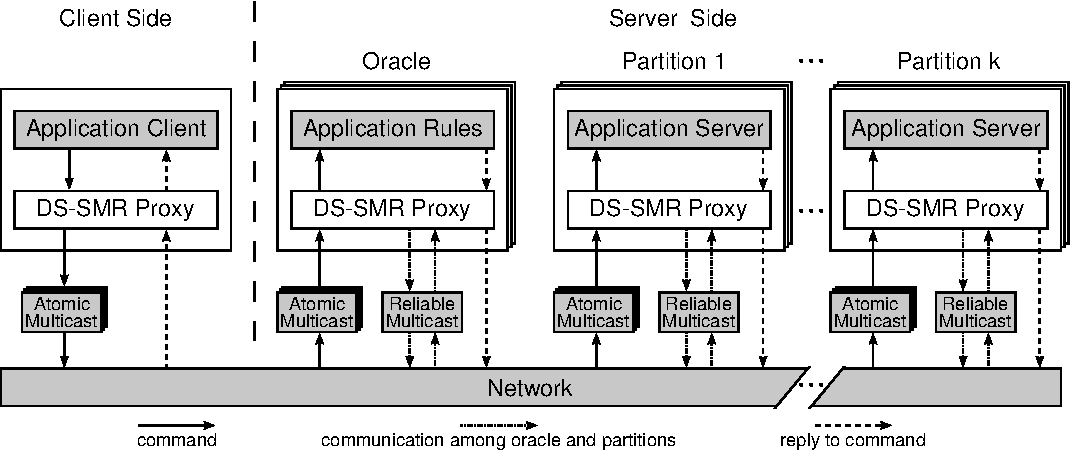
\includegraphics[width=0.8\linewidth]{figures/arch}
%\end{minipage}
%\caption{The architecture of \dssmrlong{}.}
%\label{fig:arch}
%\end{figure*}


%!TEX root =  main.tex
\section{\dynastar: dynamic and quasi-optimum state partitioning}
%\section{\dynastar: dynamic partitioning for scalable state machine replication}
%\section{The centralized partitioning scheme}

%If the system can be modeled as a graph, as described in the previous session, we can take advantage of algorithms that perform graph partitioning to optimise the state partitioning of \ssmr\  while using concepts from \dssmr. The problem of graph partitioning is well stablished and despite being NP-Complete \ref{NPC_GraphPartition}, several approximation algorithms exist. First we define what graph partitioning is and how it can analyzed to our needs, next we explore possibilities that are easily obtainable when applying the same graph's reasoning.

\subsection{Overview}
%\subsection{State partitioning as a graph problem}

\dynastar extends the decentralized dynamic scheme proposed by Long et al.~\cite{hoang2016} to cope with workloads that exhibit both strong and weak locality.
In the presence of strong locality, \dynastar converges more quickly than the decentralized dynamic scheme.
Under weak locality (i.e., workloads that cannot be perfectly partitioned), \dynastar largely outperforms the decentralized dynamic scheme.
The key insights of \dynastar are to create the workload graph on-the-fly and use graph partitioning techniques to optimally relocate application state on-demand.
\begin{itemize}
\item \emph{On-the-fly workload modeling.}
\dynastar models a service workload as a graph $G = (V, E)$, where vertices represent state variables and edges commands.
An edge connecting two variables in the graph represents a command that accesses the variables. 
The oracle builds the workload graph based on feedback from the clients and partitions, as commands are executed.
\item \emph{On-demand application state relocation.}
Periodically, the oracle computes an ``ideal" partitioning of the workload graph.
Based on this partitioning and the current location of variables, the oracle computes the destination partition for commands that access variables spread on multiple partitions.
Variables are only moved on needed, the and the destination partition strives to minimize the number of moves. 
\end{itemize}




\subsection{The \dynastar protocol}

Algorithms~\ref{alg:client_proxy}, \ref{alg:server_proxy}, and \ref{alg:oracle_proxy} describe in detail how client, server and oracle processes execute, respectively.
For brevity, we omit the delete command since the coordination involved in the execution of a create and of a delete commands are analogous. 
Moreover, in the discussion in this section, every command involves the oracle.
In the next section, we explain how clients can use a caching technique to avoid using the oracle in the execution of most commands.

\begin{figure*}
\begin{minipage}[b]{1\linewidth} % A minipage that covers the whole width of the page
\centering
      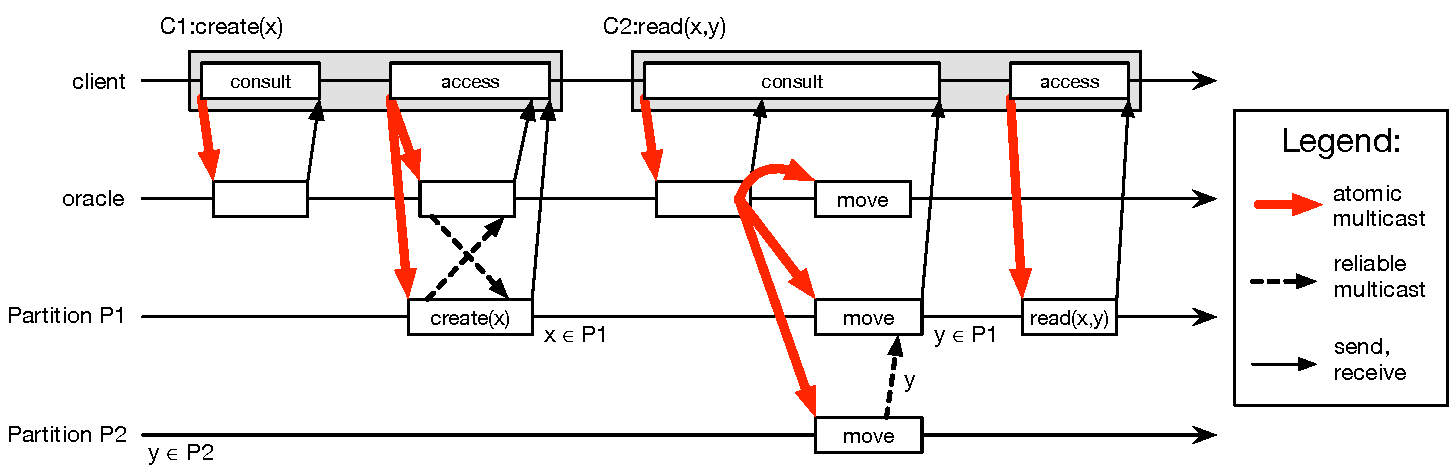
\includegraphics[width=0.9\linewidth]{figures/dynastar}
\end{minipage}
\caption{The execution of a create command and a read command in \dynastar.}
\label{fig:oracle_repartition}
\end{figure*}

%When issuing a command, the application simply forwards the command to the client proxy and waits for the reply.
%Consulting the oracle and multicasting the command to different partitions is done internally by the proxy at the client.
%Every server proxy at a server in $\ssm_i$ has only partial knowledge of the partitioning: it knows only which variables belong to $\ppm_i$.
%The oracle proxy has knowledge of every $\ppm \in \Psi$.
%To maintain such a global knowledge, the oracle must \amdel{} every command that creates, moves, or deletes variables.
%(In Section~\ref{sec:optm}, we introduce a caching mechanism to prevent the oracle from becoming a performance bottleneck.)

%\clearpage
\begin{algorithm}[h!]
\small

\begin{distribalgo}[1]

\vspace{1.0mm}

\INDENT{To issue a command $C$, the client proxy does:}

\vspace{1.0mm}

    \INDENT{\textbf{do}}
        \STATE \amcast$($oracle, $consult(C))$
        \STATE wait for $prophecy$
        \IF{$prophecy \in \{ok, nok\}$}
            \STATE $reply \leftarrow prophecy$
        \ELSE
            \STATE $C.vars \leftarrow \{v: \exists P : \langle v, P \rangle \in prophecy \}$
            \STATE $C.dests \leftarrow \{P: \exists v : \langle v, P \rangle \in prophecy \}$
            \IF{$C$ is an $access$ command and $|C.dests| > 1$}
                \STATE let $P_d$ be one of the partitions in $C.dests$
                \FOR{every $v \in C.vars$}
                    \STATE // \textit{move $v$ partition $P_d$}
                    \STATE let $P_o$ be $P : \langle v, P \rangle \in prophecy$
                    \IF{$P_o \neq P_d$}
                        \STATE $C_{move} \leftarrow move(v,P_d)$
                        \STATE $C_{move}.dests \leftarrow \{$oracle$,P_o,P_d\}$    
                        \STATE \amcast$(C_{move}.dests$, $C_{move})$
                    \ENDIF
                \ENDFOR
                \STATE $C.dests \leftarrow \{ P_s \}$
            \ENDIF
            \IF{$C$ is $create$ or $delete$}
                \STATE $C.dests \leftarrow dests \cup \{oracle\}$
            \ENDIF
            \STATE \amcast$(C.dests$, $C)$
            \STATE wait for $reply$
        \ENDIF
    \ENDINDENT
    \STATE{\textbf{while} $reply = retry$ // \textit{after $n$ retries, fall back to \ssmr}}
    \STATE return $reply$ to the application client
\ENDINDENT

\caption{\dssmr\ Client Proxy}
\label{alg:client_proxy}
\end{distribalgo}
\end{algorithm}
\begin{algorithm}[h!]
\small

\begin{distribalgo}[1]

\vspace{1.0mm}

\INDENT{To execute a command $C$, the server proxy in partition $\ppm$ does:}

    \vspace{1.0mm}
    
    \INDENT{\textbf{when} \rmdel$( \langle val, C \rangle )$}
        \STATE $rcvd\_msgs \leftarrow rcvd\_msgs \cup \{\langle val, C \rangle\}$
    \ENDINDENT

    \vspace{1.0mm}

    \INDENT{\textbf{when} \amdel$(C)$}

    \vspace{1.0mm}

        \IF{\underline{$C$ is an $access(\omega)$ command}}
            \IF{$\exists v \in \omega : v \not\in \ppm$}
                \STATE reply with $retry$
            \ELSE
                \STATE have the command executed by the application server
                \STATE send the reply to the client
            \ENDIF
        

        \vspace{1.0mm}
    
        \ELSIF{\underline{$C$ is a $move(v,\ppm_s,\ppm_d)$ command}}
            \IF{$\ppm = \ppm_s$}
                \IF{$v \in \ppm$}
                    \STATE \rmcast$(\ppm_d$,$\langle v, C \rangle)$
                    \STATE $\ppm \leftarrow \ppm \setminus \{v\}$
                \ELSE
                    \STATE \rmcast$(\ppm_d$,$\langle null, C \rangle)$
                \ENDIF
            \ELSE
                \STATE wait until $\exists val : \langle val, C \rangle \in rcvd\_msgs$
                \IF{$val \neq null$}
                    \STATE $v \leftarrow val$
                    \STATE $\ppm \leftarrow \ppm \cup \{v\}$
                \ENDIF
            \ENDIF
        
        \vspace{1.0mm}
    
        \ELSIF{\underline{$C$ is a $create(v)$ command}}
            \STATE wait until $\langle val, C \rangle \in rcvd\_msgs$
            \IF{$val = ok$}
                \STATE $\ppm \leftarrow \ppm \cup \{v\}$
%                \STATE reply with $success$
%            \ELSE
%                \STATE reply with $retry$
            \ENDIF
        
        \vspace{1.0mm}
        
        \ELSIF{\underline{$C$ is a $delete(v)$ command}}
            \IF{$v \in \ppm$}
                \STATE $\ppm \leftarrow \ppm \setminus \{v\}$
%                \STATE reply with $success$
%            \ELSE
%                \STATE reply with $retry$
            \ENDIF
        \ENDIF
    \ENDINDENT
\ENDINDENT

\caption{\dssmr\ Server Proxy}
\label{alg:server_proxy}
\end{distribalgo}
\end{algorithm}
\begin{algorithm}[t!]
\small

\begin{distribalgo}[1]

%\vspace{1.0mm}

	\INDENT[\textbf{Task 1}]{\colorbox{\coloralgo}{\textbf{when} \amdel$(consult(C))$}}
%		\INDENT{\textbf{case} $C$ is a $consult(C_c)$ command:}
%			\STATE $update(G_W, \omega)$
			\INDENT{\textbf{case} $C$ is a $create(v)$ command:}
				\IF[if $v$ already exists...]{$\parts(\{v\}) \neq \bot$}
					\STATE $prophecy \leftarrow nok$
					\COMMENT{...notify client}
				\ELSE[if $v$ doesn't exist...]
					\STATE $\ppm \leftarrow target(G_W, \{v\})$
					\COMMENT{...determine $v$'s partition}
					\STATE $prophecy \leftarrow (\{ \ppm, oracle \}, false)$
%					\COMMENT{prepare client's response}
				\ENDIF
			\ENDINDENT
			\INDENT{\textbf{case} $C$ is an $access(\omega)$ command:}
				\IF[if $v$ doesn't exist:]{$\exists v \in \omega : \parts(\{v\}) = \bot$}
					\STATE $prophecy \leftarrow nok$
					\COMMENT{tell the client}
				\ELSE[if all vars in $\omega$ exist]
%					\STATE $dests \leftarrow \emptyset$
%					\FOR{each $v \in \omega$}
%						\STATE $dests \leftarrow dests \cup partition(v)$
%					\ENDFOR
					\STATE $dests \leftarrow \parts(\omega)$
					\COMMENT{get all partition involved}
					\IF[if only one partition:]{$|dests| = 1$}
						\STATE $prophecy \leftarrow (dests,false)$
%						\COMMENT{tell client which partition}
					\ELSE[if multiple partitions involved]
						\STATE $\ppm_d \leftarrow target(G_W, \omega)$
						\COMMENT{$\ppm_d$ will store all vars in $\omega$}
						\STATE $alldest \leftarrow \{oracle\} \cup dests$
						\COMMENT{move $v$ from $\ppm_s$...}
						\STATE \amcast$(alldest, move(\omega,dests,\ppm_d))$
						\COMMENT{...to $\ppm_d$}						
%						\FOR[for each involved var $v$]{each $v \in \omega$}
%							\STATE $\ppm_s \leftarrow \parts(\{v\})$
%							\COMMENT{$\ppm_s$ is $v$'s current partition}
%							\IF[if $v$ not in $\ppm_d$:]{$\ppm_s \neq \ppm_d$}
%								\STATE $aux \leftarrow \{oracle,\ppm_s,\ppm_d\}$
%								\COMMENT{move $v$ from $\ppm_s$...}
%								\STATE \amcast$(aux$, $move(v,\ppm_s,\ppm_d))$
%								\COMMENT{...to $\ppm_d$}
%							\ENDIF 
%						\ENDFOR
						\STATE $prophecy \leftarrow (\{\ppm_d\},true)$
					\ENDIF 
				\ENDIF
			\ENDINDENT
			\STATE send $prophecy$ to the client
%			\INDENT{\textbf{case} $C_c$ is a $delete(v)$ command:}
%				\IF{$partition(v) = \bot$}
%					\STATE $prophecy \leftarrow ok$
%				\ELSE
%					\STATE $prophecy \leftarrow (\{ \ppm : v \in \ppm, oracle \}, -)$
%				\ENDIF
%			\ENDINDENT
%		\ENDINDENT
	\ENDINDENT
	\vspace{1.0mm}

	\INDENT[\textbf{Task 2}]{\colorbox{\coloralgo}{\textbf{when} \amdel$(create(v))$}}
%	\INDENT{\textbf{case} $C$ is a $create(v)$ command:}
		\STATE let $\ppm_c \in C.dests \setminus \{oracle\}$
		\COMMENT{var created in $\ppm_c$}
		\STATE \rmcast$(\ppm_c, \langle signal, C \rangle )$
		\COMMENT{exchange signal to...}
		\STATE wait until $\langle signal, C \rangle \in rcvd\_msgs$
		\COMMENT{...coordinate partitions}
		\STATE $\ppm_c \leftarrow \ppm_c \cup      \{v\}$
                \STATE send $ok$ to the client
	\ENDINDENT

	\vspace{1.0mm}
	\INDENT[\textbf{Task 3}]{\colorbox{\coloralgo}{\textbf{when} \amdel$(move(\omega,dests,\ppm_d))$}}
%        \INDENT{\textbf{case} $C$ is a $move(v,\ppm_s,\ppm_d)$ command:}
                \STATE \textbf{for} each $\ppm_s \in dests$ \textbf{do} $\ppm_s \leftarrow \ppm_s \setminus \omega$
                \COMMENT{update partitions...}
                \STATE $\ppm_d \leftarrow \ppm_d \cup \omega$
                \COMMENT{...and add new variables}
                \STATE send $ok$ to the client
	\ENDINDENT

        \vspace{1.0mm}
    
	\INDENT[\textbf{Task 4}]{\colorbox{\coloralgo}{\textbf{when} \rmdel$( \langle val, C \rangle )$}}
		\STATE $rcvd\_msgs \leftarrow rcvd\_msgs \cup \{\langle val, C \rangle\}$
	\ENDINDENT
	
	\vspace{1.0mm}
	\INDENT{\colorbox{\coloralgo}{\textbf{function} \parts$(vars)$}}
		\STATE $aux \leftarrow \{ \ppm : \exists v \in vars \cap \ppm \}$
		\STATE return $aux$
	\ENDINDENT
	
%	\vspace{1.0mm}
	\rule{83mm}{0.4pt}
%	\vspace{0.1mm}

	\INDENT[\textbf{Task 5}]{\colorbox{\coloralgo}{\textbf{when} \amdel$(hint(V_h,E_h))$}}
		\STATE update $G_W$ with $(V_h,E_h)$
%		\STATE send $ok$ to the client
	\ENDINDENT
	
	\vspace{1.0mm}
    
	\INDENT[\textbf{Task 6}]{\colorbox{\coloralgo}{\textbf{periodically} do}}
		\STATE compute ideal partition $\ip_1, ..., \ip_m$ from $G_W$
	\ENDINDENT
	
	\vspace{1.0mm}
    
	\INDENT{\colorbox{\coloralgo}{\textbf{function} target$(vars)$}}
		\STATE $\ppm \leftarrow$ compute destination partition for $vars$ from\\ \hspace{8mm}current $\ppm_1, ..., \ppm_m$ and ideal $\ip_1, ..., \ip_m$ partitionings
		\STATE return $\ppm$
	\ENDINDENT	
	
%	\vspace{1.0mm}
%        
%	\INDENT{\textbf{case} $C$ is a $delete(v)$ command:}
%		\STATE let $\ppm_d$ be $\ppm : \{\ppm\} = C.dests \setminus \{$oracle$\}$
%		\STATE $\ppm_c \leftarrow \ppm_c \setminus      \{v\}$
%		\STATE \rmcast$(\ppm_c, \langle ok, C \rangle )$
%			\STATE wait until $\exists val : \langle val, C \rangle \in rcvd\_msgs$
%	\ENDINDENT

%\ENDINDENT

\caption{Oracle}
\label{alg:oracle_proxy}
\end{distribalgo}
\end{algorithm}



\subsubsection{The client process} 

To execute a command, the client atomically multicasts the command to the oracle in a consult message to find out the partitions involved.
The oracle replies with a prophecy, which may already tell the client that the command cannot be executed (e.g., it needs a variable that does not exist, it tries to create a variable that already exists).
If the command can be executed, the client receives a prophecy containing a tuple $(dests, sync)$, where $dests$ is a set of the partitions the command must be atomically multicast to for execution, and $sync$ is a flag that tells the client whether it must coordinate with a partition before atomically multicasting the command.
This happens if the oracle requests variables to be moved to a single destination partition, in which case the client must wait for the destination partition to receive the variables.

After the client atomically multicasts the command to the destination partition, it waits for a response from the servers in the partition.
The client must retry the command if the partition cannot execute the command.
This happens if some of the variables needed by the command were moved to another partition due to other commands. 
To ensure that a command is eventually executed, after retrying a few times, the client falls back \ssmr{}, multicasting the command to all partitions (and the oracle, in case of a create or delete command).

\subsubsection{The server process} 

When a server delivers a command for execution, it first checks that all variables accessed by the command are stored locally, in which case the command is executed and the response is sent back to the client (Task 1 in Algorithm~\ref{alg:server_proxy}).
If one or more variables are not stored at the partition, the server returns a message to the client to retry the operation.
This happens if some variables have been moved to another partition due to another command. 

Upon delivering a message to move variables (Task 2), a server in the source partition reliably multicasts all the needed variables stored locally to the destination partition (possibly none, if these variables have already been moved).
Servers in the destination partition simply wait for a message from each source partition.

When a server delivers a message to create a variable (and similarly to delete an existing variable), it coordinates with the oracle (Task 3).
The exchange of signals between the partition where the variable will be created and the oracle ensures that interleaved executions between create and delete commands will not lead to violations of linearizability (i.e., this is essentially the execution of a multi-partition command involving the oracle and a partition~\cite{bezerra2014ssmr}).

\subsubsection{The oracle} 

When the oracle delivers a consult request (Task 1 in Algorithm~\ref{alg:oracle_proxy}), it distinguishes between two cases.
\begin{itemize}
\item If the command is to create a variable $v$, the oracle checks that the $v$ does not already exist, in which case the oracle determines the destination partition of $v$ and returns a response to the client.
In the case of a create, the oracle chooses a random partition for the new variable.
\item If the command is not a create, the oracle first checks that all variables involved in the command exist.
If the variables exist and they are all in a single partition, the oracle returns to the client a prophecy with the partition the command must be atomically multicast to for execution.
If the variables accessed by the command are distributed in multiple partitions, the oracle determines the destination partition and atomically multicasts a move command to all such partitions and to the destination partition.
\end{itemize}

The oracle executes a create command (Task 2) by updating its partition information and coordinating with the destination partition of the variable.
This is done to avoid interleaved executions with other commands, which could lead to consistency violations. 
To execute a move command (Task 3), the oracle simply updates its local information about source and destination partitions.
In the case of a move command, the oracle does not coordinate with the involved partitions.
This is not necessary because a move cannot interleave its execution with a create and interleaved executions with other move commands simply result in retries by the clients.

The oracle also keeps track of the workload graph, periodically computes the ``ideal" partitioning of the graph, and determines the destination partition for move operations.
To maintain the workload graph (Task 5), the oracle receives hints with variables (i.e., vertices in the graph) and executed commands (i.e., edges in the graph).
These hints can be submitted by the clients (e.g., after the execution of a command), or by the partitions, which collect data upon executing commands and periodically inform the oracle.
In our social network application, clients inform the oracle upon submitting ``structural operations" on the social graph, that is, operations that change the  graph (i.e., follow and unfollow requests).

To ensure that the ideal partitioning periodically computed by the oracle replicas is deterministic (Task 6), each replica triggers the partitioning upon delivering a constant number of hints.
Moreover, the algorithm used to compute the partitioning of the graph must be also deterministic.
To determine the destination partition of a set of variables, as part of a move, the oracle chooses the partition that results in the minimum number of variables that need to be moved given the ideal partitioning and the current location of the variables.

\subsection{Performance optimizations}
\label{sec:optm}

In the algorithm presented in the previous section, clients always need to consult the oracle to determine the partition a command must be atomically multicast to for execution.
Obviously, if every command involves the oracle, the system is unlikely to scale, as the oracle will likely become a bottleneck.
To address this issue, clients are equipped with a location cache.
Before submitting a consult request to the oracle, the client checks its location cache.
If the cache contains the partition of the variables needed by the command and all variables are in a single destination partition, the client can atomically multicast the command to the partition and avoid contacting the oracle. 

The client needs to contact the oracle if not all variables needed by the command are in the same partition, or if the cache contains outdated information, or the command is a create, in which case it must involve the oracle, as explained before.
If the cache contains outdated information and the addressed partition does not contain all the variables accessed by the command, the partition tells the client to retry the command.
In this case, the client contacts the oracle and then updates its cache with the oracle's response.


\subsection{Correctness}
\label{sec:correctness}

In this section, we argue that \dssmr\ ensures termination and linearizability.
By ensuring termination, we mean that for every command $C$ issued by a correct client, a reply to $C$ different than $retry$ is eventually received by the client.
This assumes that at least one oracle process is correct and that every partition has at least one correct server.
Given these constraints, the only thing that could prevent a command from terminating would be an execution that forced the client proxy to keep retrying a command.
This problem is trivially solved by falling back to \ssmr\ after a predefined number of retries: at a certain point, the client proxy multicast the command to all server and oracle processes, which execute the command as in \ssmr{}, i.e., with coordination among all partitions and the oracle.

As for linearizability, we argue that, if every command in execution \ex\ of \dssmr\ is delivered by atomic multicast and is \emph{execution atomic} (as defined in~\cite{bezerra2014ssmr}), then \ex\ is linearizable.
We denote the order given by atomic multicast by relation $\prec$.
Given any two messages $m_1$ and $m_2$, ``$m_1 \prec m_2$'' means that there exists a process that delivers both messages and $m_1$ is delivered before $m_2$, or there is some message $m'$ such that $m_1 \prec m'$ and $m' \prec m_2$, which can be written as \mbox{$m_1 \prec m' \prec m_2$}.
%\fxnote[draft]{use the phrase \"there exists a process that\" }
Also, for the purposes of this proof, we consider the oracle to be a partition, as it also \amdel{}s and executes application commands.

Suppose, by means of contradiction, that there exist two commands $x$ and $y$, where $x$ finishes before $y$ starts, but $y \prec x$ in the execution.
There are two possibilities to be considered: (i) $x$ and $y$ are delivered by the same process $p$, or (ii) no process delivers both $x$ and $y$.

In case (i), at least one process $p$ delivers both $x$ and $y$.
As $x$ finishes before $y$ starts, then $p$ delivers $x$, then $y$. From the properties of atomic multicast, and since each partition is mapped to a multicast group, no process delivers $y$, then $x$.
Therefore, we reach a contradiction in this case.

In case (ii), if there were no other commands in \ex, then the execution of $x$ and $y$ could be done in any order, which would contradict the supposition that $y \prec x$.
Therefore, there are commands $z_1, ..., z_n$ with atomic order $y \prec z_1 \prec \cdots \prec z_n \prec x$, where some process $p_0$ (of partition $\ppm_0$) delivers $y$, then $z_1$; some process $p_1 \in \ppm_1$ delivers $z_1$, then $z_2$, and so on: process $p_i \in \ppm_i$ delivers $z_{i}$, then $z_{i+1}$, where $1 \leq i < n$.
Finally, process $p_n \in \ppm_n$ delivers $z_n$, then $x$.

Let $z_0 = y$ and let $atomic(i)$ be the following predicate:
``For every process $p_i \in \ppm_i$, $p_i$ finishes executing $z_i$ only after some $p_0 \in \ppm_0$ started executing $z_0$.''
We now claim that $atomic(i)$ is true for every $i$, where $0 \leq i \leq n$.
We prove our claim by induction.






%!TEX root =  main.tex
\section{Implementation}
\label{sec:implementation}


Our  \dynastar prototype is written as a
Java \red{8?} library.
All code, including the experiment harness,
is publicly available with an open-source
license.\footnote{https://github.com/anonymous}
Application designers who use \dynastar
 to implement a replicated service must extend three key classes:
 \begin{itemize}
 \item[--] \emph{PRObject}: provides a common interface for (partially) replicated data items.
 \item[--] \emph{PartitionStateMachine}: encapsulates the logic of the server
   proxy. Note that the server logic is written without knowledge of the actual partitioning scheme. The \dynastar library
   handles all communication between partitions and the oracle transparently.
 \item[--] \emph{OracleStateMachine}: computes the mapping of objects to partitions.
Our default implementation uses the \red{METIS library} to provide an optimal partitioning based on the workload graph.
 \end{itemize}

 We note one important implementation detail.  The oracle is
 multi-threaded, and can service requests while computing a new
 partitioning concurrently. To ensure that all replicas start using
 the new partitioning consistently, the oracle identifies each
 partitioning with a unique id.  When an oracle replica finishes a
 repartitioning, it atomically multicasts the id of the new
 partitioning to all replicas of the oracle.  The first delivered id
 message defines the order of the new partitioning with respect to
 other oracle operations.





%% In this section, we describe \libname{}, a library that implements
%% both \ssmr{}, \dssmr{} and \dynastar{}.  We also present \appname{}, a
%% scalable social network application built with
%% \libname{}. \libname\ and \appname\ were both implemented in Java.

%% \subsection{\libname}

%% \libname{} implements functionalities of static and dynamic mapping,
%% and supports centralized and decentralized partitioning schemes.
%% There are three classes that the developer (i.e., application
%% designer) must extend to implement a replicated service with
%% \libname{}: PRObject, PartitionStateMachine, OracleStateMachine.

%% The \emph{PRObject class} represents any kind of data item that is
%% part of the service state. The state is partially replicated (i.e.,
%% objects are distributed among partitions). Therefore, when executing a
%% command, a replica might not have local access to some of the objects
%% involved in the execution of the command. The developer informs
%% \libname{} which object classes are partially replicated by extending
%% the PRObject class. Each object of such a class is stored locally or
%% remotely, but the application code is agnostic to the location of an
%% object. All calls to methods of such objects are intercepted by
%% \libname{}, transparently to the developer.

%% The \emph{PartitionStateMachine class} represents logic of the server
%% proxy. The application server class must extend the
%% PartitionStateMachine class. To execute commands, the developer must
%% provide an implementation for the method executeCommand(Command). The
%% code for such a method is agnostic to the existence of partitions. In
%% other words, developer programs for classical state machine
%% replication (i.e., full replication). \libname{} is responsible for
%% handling all communication between partitions and oracle
%% transparently. Objects that are involved in application's command will
%% be available to the partition at the time it is accessed by the
%% partitions. To start the server, method runStateMachine() is
%% called. Method createObject() also needs to be implemented, where the
%% developer defines how new state objects are loaded or created.


%% The \emph{OracleStateMachine class} defines the oracle, which is
%% deployed as a partition.  Because the oracle is in charge of moving
%% the PRObjects to the appropriate partitions, it requires a partitioner
%% that will provide for each object a desired location. A default
%% partitioner is implemented using METIS, a state-of-the-art graph
%% partitioner, but any algorithm that takes as input a graph and outputs
%% a mapping of objects to partitions is a valid partitioner.  The
%% workload graph is built by aggregating hints about the objects' access
%% patterns, and the mapping it returns indicates the ideal partition for
%% each object. Since the partitioner is executed in every oracle
%% replica, its output should be deterministic so all the replicas
%% transition to the same state after the partitioning.  The developer
%% can override the default algorithm to partition the graph and the
%% oracle is agnostic to its internal behavior.  At any time, the
%% application can request a repartitioning of the graph.


\subsection{\appname}
\label{sec:imp:\appname}

For the purposes of our evaluation, we have developed a Twitter-like
service named \appname{} using the \dynastar{} library.  With
\appname, users can follow, unfollow, post, or read other users'
tweets according to whom the user is following. Like Twitter, users
are constrained to posting 140-character messages.

Given that users in social networks spend most of the time reading
(i.e., performing getTimeline) \cite{facebookTAO}, we designed
\appname\ so that getTimeline are always a single-partition command.
Thus, when a user request a timeline, all posts are available in the
user's partition.  As a consequence, post, follow or unfollow commands
can lead to object moves.  Follow and unfollow commands can involve at
most two partitions, while posts can require object moves from one or
more partitions.


\subsection{Alternative Systems}

Throughout our evaluation, we compare \dynastar{} to two alternative
systems: S-SMR and DS-SMR. For performing our experiments, we used
the implementations of the two systems that are available in public
repositories. Since all three systems (S-SMR, DS-SMR, and Dynastar) provide
a common application-level interface, there was no additional work required
to port the \appname{} application. \rjs{We should add links to the repositories.}

%!TEX root =  main.tex
\section{Performance evaluation}
\label{sec:experiments}

In this section, we evaluate \dynastar{} according to various metrics,
under a variety of different operational parameters.  As a
representative application, we use the \appname{} social networking
service described in the previous section.  As a point of comparison,
we perform the same experiments with both
\ssmr{}~\cite{bezerra2014ssmr} and \dssmr. Our experiments show that
\dynastar{} is able to rapidly adapt to changing workloads, while
achiving throughputs and latencies far better than the existing
state-of-the-art approaches to partitioning.


\subsection{Experiemental environment}
\label{sec:evaluation:setup}

We conducted all experiments on a cluster with two types of nodes: (a)
HP SE1102 nodes, equipped with two Intel Xeon L5420 processors running
at 2.5 GHz and with 8 GB of main memory, and (b) Dell SC1435 nodes,
equipped with two AMD Opteron 2212 processors running at 2.0 GHz and
with 4 GB of main memory. The HP nodes were connected to an HP
ProCurve 2920-48G gigabit network switch, and the Dell nodes were
connected to another, identical switch. Those switches were
interconnected by a 20 Gbps link.  All nodes ran CentOS Linux 7.1 with
kernel 3.10 and had the OpenJDK Runtime Environment~8 with the
\mbox{64-Bit} Server VM (build 25.45-b02).


\subsection{Methodology and goals}
\label{sec:evaluation:methodology}

The experiments explore the following questions:
\begin{itemize}
\item \emph{How does \dynastar compare to other approaches?} 
\item \emph{How does the number of partitions affect the performance of posts for a fixed social graph?}
\item \emph{How does \dynastar perform under dynamic workloads?}
\item \emph{When will the oracle become a bottleneck?}
\end{itemize}



\paragraph*{Social network graph creation}
%
To generate the social graphs used in the experiments, we used the
Holme-Kim model~\cite{holme-kim}.  We created power-law graphs (also
known as scale-free graphs) with a clustering coefficient varying from
0.6 to 1, which represent the geometric structures of social
networks. The coefficient is the probability that whenever an edge
$(v, w)$ is added to the graph, $v$ connects to some neighbour of $w$.
In the experiments, we tested graphs with 10000 users. We characterize
different workloads by varying the percentage of edge-cuts.  For
example, a graph with a 5\% edge cut means that 5\% of the total edges
in the graph have connected vertices located in different partitions.
Graphs with some percentage of edge-cuts have \emph{weak locality}.

\paragraph*{Command generation}
%
As a workload for the social graph, clients issued a sequence of post
commands.  For each command, the client selects a random node as
the poster.  We focused on post commands, since they may access
multiple partitions.  We used 100 clients per partition. In other
words, the number of clients varied linearly with the number of
partitions.  Each client repeatedly issued synchronous post commands,
waiting for a response from the storage.

\begin{figure*}[ht!]
	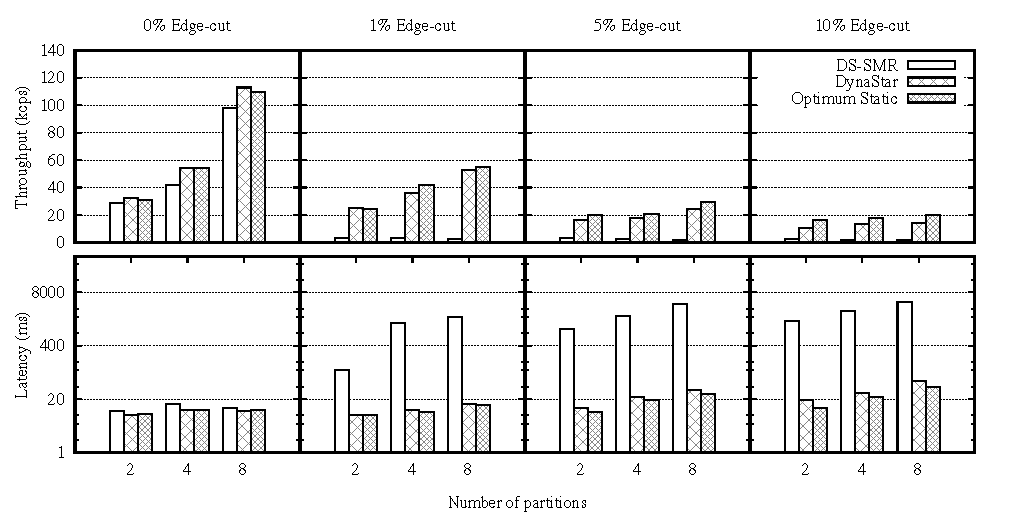
\includegraphics{figures/experiments/throughput-latency-avg-all}
	\caption{Throughput and latency, varying edge-cuts for different partitioning size}
	\label{fig:varying_edge_cut}
\end{figure*}



\paragraph*{Performance metrics}
%
The latency was measured as the end-to-end time between issuing the
command, and receiving the response.  Throughput was measured as the
number of posts/second that the clients were able to send.

\paragraph*{Operational parameters}
%
With post commands, the frequency of single-partition
vs. multi-partition commands depends on the number of partitions, the
geometry of the social graph, and the technique used to partition the
data. We ran experiments with 2, 4, and 8 partitions.  To vary the
geometry, we generated graphs with varying percentages of edge-cuts as
computed by METIS on a static graph. Our experiments used graphs with
0\%, 1\%, 5\% and 10\% of edge cuts. As already mentioned, we compared 
three strategies: \ssmr{}, \dssmr, and \dynastar.


\subsection{\dynastar vs. alternative systems}
\label{sec:evaluation:results}

Figure~\ref{fig:varying_edge_cut} shows the throughput and latency of the three strategies, as we vary the number of partitions for social networks with different percentages of edge cuts.
As expected, all three techniques perform similarly on tests with
strong locality, because there are no cross-partition commands after
the graph is perfectly partitioned and no more moves occur in
\dynastar or \dssmr.  Also, no synchronization among partitions is
necessary for \ssmr.
Consequently, all three schemes scale remarkably well.
Although \dynastar and DS-SMR have comparable performance, they differ in an important way. 
As shown in Figure~\ref{fig:motivation} (top left graph) for 4 partitions, \dynastar converges to maximum throughput after 30 seconds from the beginning of the execution, while it takes DS-SMR (decentralized dynamic scheme) about 90 seconds to converge.


%To compare \dynastar with alternative approaches, we measured the
%throughputh and latency for a varying number of partitions and a
%varying percentage of edge-cuts. The results are shown in
%Figure~\ref{fig:varying_edge_cut}.

With social networks that exhibit weak locality (edge cut percentage greater than zero) \dssmr\ performance decreases significantly.  
This happens because with weak locality, objects in \dssmr\ are constantly being moved back and forth between partitions without converging to a stable configuration (see also Figure~\ref{fig:motivation}, graph on the bottom right, for 4 partitions). 
In contrast, for \dynastar and \ssmr with an optimized partitioning, we see that the throughput scales with the number of partitions up to 10\% of edge cuts. 
With 10\% of edge cuts and above, the overhead from moves (in \dynastar) and cross-partition commands (in S-SMR) outweight the gains from additional partitions.

We can draw similar results about the latency of the three strategies (Figure~\ref{fig:varying_edge_cut}, graphs on the bottom).
The large number of move operations in DS-SMR with social graphs that cannot be perfectly partitioned result in increased latency.

\subsection{Performance with the number of partitions}
\label{sec:evaluation:results}

While in the previous section we considered executions where the percentage of edge cuts is fixed as the number of partitions increases, we now consider the performance of \dynastar when a fixed social graph is partitioned 

In this tests we measure the throughput of the same graph partitioned in different
partition sizes. As seen in Figure~\ref{fig:4p1p_varying_partition_size}, the throughput
scales with the number of partitions up until a point, then decreases, that is because
when increasing the partitioning size, the number of edge-cuts also increase, in this
case, the number of edge-cuts for 2, 4, 6 and 8 partitions were respectively 
0.13\%, 1.06\%, 2.28\% and 2.67\%. \ef{Is that reason enough?}

\begin{figure}[ht]
	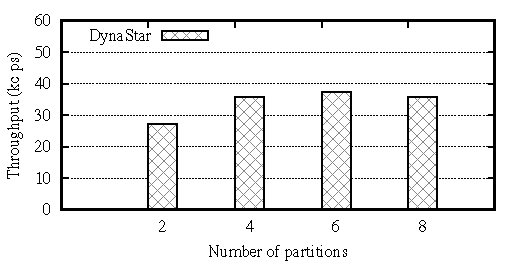
\includegraphics{figures/experiments/throughput-avg-vary-partition}
	\caption{Same graph in different partitioning}
	\label{fig:4p1p_varying_partition_size}
\end{figure}


\subsection{Performance under dynamic workloads}

Figure~\ref{fig:dynamic_load_tput} depicts dynamically repartitioning
on-the-fly.  We started the system with an empty graph. Then clients
continuously create users and links between them during the experiment
(running the follow command).  The oracle monitors changes in the
graph's structure and trigger a repartitioning when the number of
changes exceed a threshold.  Each time the repartitioning took place,
the partitioning became better, that helps the throughput increase.

\begin{figure}[ht]
	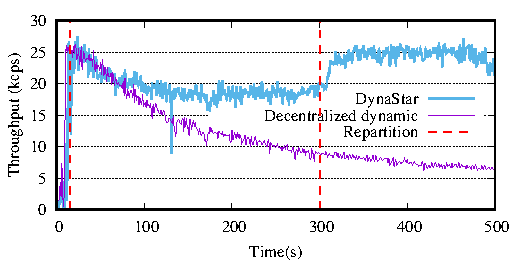
\includegraphics{figures/experiments/dynamicload-tp-move-4p}
	\caption{Adding nodes and repartitioning dynamically}
	\label{fig:dynamic_load_tput}
\end{figure}

\subsection{The performance of the oracle}

\dynastar differs from \dssmr in that it uses a centralized oracle
that maintains a global view of the workload graph. This oracle allows
\dynastar to make better choices about data movement, resulting in overall
better throughput and lower latency. However, introducing centralized
components in a distributed system is always a cause for some skepticism,
in case the component becomes a bottleneck. We therefore conducted two
experiments to evaluate if the \dynastar oracle is a bottleneck to
system performance. The results show that the load on the oracle is
low, suggesting that \dynastar scales well.


The first experiment assesses the scalability of the static METIS algorithm
in isolation. We measured the time to compute the partitioning solution, and
the memory usage of the algorithms for increasingly large graphs. 
The results, shown in Figure~\ref{fig:metis_size_time}, shows that METIS scales
linearly in both memory and computation time on graphs of up to 10 million vertices.


\begin{figure}[ht!]
  \centering
    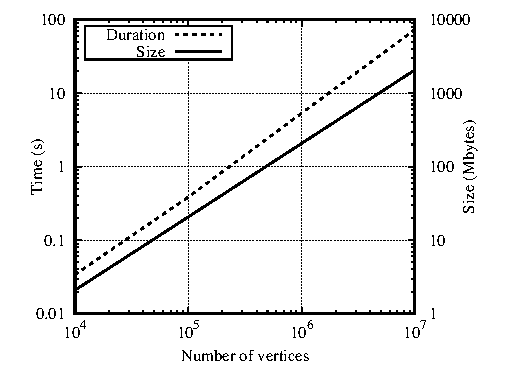
\includegraphics[width=\columnwidth]{figures/metis_size_time}
	\caption{METIS processor and memory usage}
	\label{fig:metis_size_time}
\end{figure}

The second experiment evaluates the oracle in terms of CPU load over
time, for varying numbers of partitions. The results are shown in
Figure~\ref{fig:cpu_oracle}. The plot shows that load is higher in the
beginning of the experiment, when the clients had not yet cached the
requests. However, the load diminishes rapidly, and remains relatively
low over time. This is because access to the oracle is necessary only
when clients have an invalid log or when a repartition happens. This experiments
suggest that the oracle would not become a bottleneck for reasonably large
deployments.

\begin{figure}[ht]
	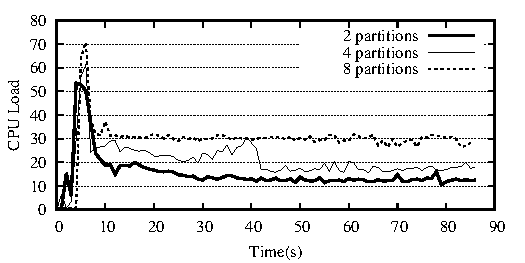
\includegraphics{figures/experiments/oracle-load}
	\caption{CPU load in the oracle}
	\label{fig:cpu_oracle}
\end{figure}


\section{Related work}
\label{sec:rw}

State machine replication~\cite{Lam78, Sch90, Kapritsos:2012um, kotla2004htbft, santos2013htsmr} is known for its strong consistency guarantees, which comes from the assumption of deterministic execution.
Its drawback is that such a determinism is usually ensured by having every replica executing the same commands, in the same order---that is, sequentially.
Since consistent ordering is fundamental for SMR, some authors proposed to optimize the ordering and propagation of commands (i.e., the atomic broadcast layer of the system).
For instance, \cite{kapritsos2010scalable} proposes to divide the ordering of commands between different clusters: each cluster orders only some requests, and then forwards the partial order to every server replica, which then merges the partial orders deterministically into a single total order that is consistent across the system.
In~\cite{biely2012spaxos}, Paxos~\cite{Lamport:1998ea} is used to order commands, but it is implemented in a way that avoids overloading the leader process, which would turn it into a bottleneck.

Multi-threaded execution is a potential source of non-determinism, depending on how threads are scheduled to be executed in the operating system.
Some works attempted to circumvent this problems and come up with a multi-threaded, yet deterministic implementation of SMR.
In \cite{santos2013htsmr}, the authors propose to parallelize the receival and dispatching of commands, while still executing commands sequentially.
In \cite{kotla2004htbft}, application semantics is used to determine which commands can be executed concurrently and still produce a deterministic outcome (e.g., read-only commands).
In \cite{Kapritsos:2012um}, commands are tentatively executed in parallel.
After the parallel execution, replicas verify whether they reached a consistent state; if not, commands are rolled back and re-executed sequentially.

Many database replication schemes aim at achieving higher throughput by relaxing consistency, that is, they do not ensure linearizability.
In deferred-update replication \cite{sciascia2012sdur, chundi96dur, kobus2013hybrid, SousaOMP01}, replicas commit read-only transactions immediately, not always synchronizing with each other.
Although this indeed improves performance significantly, it allows non-linearizable executions to take place; database systems usually ensure serializability \cite{BHG87} or snapshot isolation \cite{LinKJPA09}.
Those criteria can be considered weaker than linearizability, in the sense that they do not take into account real-time precedence of different commands among different clients. 
For some applications, these consistency levels may be enough, allowing the system to scale better, but services that require linearizability cannot be implemented with such techniques.

Efforts to make linearizable systems scalable have been made in the past~\cite{corbett2013spanner, bezerra2014ssmr, le2016dssmr, Glendenning2011, Marandi11}.
In \cite{Glendenning2011}, the authors propose a scalable key-value store based on DHTs, ensuring linearizability, but only for requests that access the same key. 
In \cite{Marandi11}, a partitioned variant of SMR is proposed.
However, it requires total order (i.e., all commands have to be ordered against each other) and it does not allow a single command to update variables in different partitions.
Spanner~\cite{corbett2013spanner} uses a separate Paxos group per partition and, to ensure strong consistency across partitions, clocks are assumed to be synchronized.
Although the authors say that Spanner works well with GPS and atomic clocks, if clocks go out of synch beyond the tolerated difference, correcteness is not guaranteed.
\ssmr{}~\cite{bezerra2014ssmr} ensures consistency across partitions without any assumption about clock synchronization, but relying on a static partitioning of the state.
\dssmr{}~\cite{le2016dssmr} extends S-SMR by allowing state variables to migrate across partition in order to reduce multi-partition commands.
However, \dssmr{} implements repartitioning in a very simple way that does not perform very well in scenarios with weak locality.
\dynastar\ improves on DS-SMR by employing well known graph partitioning techniques to decide where each variable should be.
Moreover, \dynastar\ dillutes the cost of repartitioning by moving variables on-demand, that is, only when they are accessed by some command.

\eb{I'm not sure if this paragraph should stay here; I'd vote to remove it...}
\dynastar\ is not to be confused with other dynamic replication schemes though.
Systems such as~\cite{birman2010dsr,guessoum2003dar,dustdar2007soc} are ``dynamic'' in the sense that they allow the membership to be reconfigured during execution.
For instance, a multicast layer based on Paxos can be reconfigured by adding or removing acceptors. They also allow server replicas to be added and removed during execution.
However, this is orthogonal to what \dynastar\ proposes.
\dynastar\ consists of allowing the \emph{state partitioning}, that is, which state variables belong to which partition, to change dynamically.
The greatest challenge that is addressed by \dynastar\ is how to provide such a solution, with a dynamic partitioning oracle, while ensuring a very strong level of consistency (linearizability), as variables are created, deleted, and moved across partitions, based on the access patterns of the workload.

Graph-partitioning is an interesting problem with many proposed solutions~\cite{Abou-Rjeili:2006,kernighan1970efficient,hendrickson2000graph}.
In this work, we do not introduce a new graph partitioning solution, but instead we use a well-known one (Metis~\cite{Abou-Rjeili:2006}) to partition the state of a service implemented with state machine replication.
Similarly to \dynastar{}, Schism~\cite{curino2010sch} also uses graph-based partitioning to decide where to place data items in a transactional database.
The authors propose to use the workload to create a graph that captures dependencies between data items, but not much detail is given about how the repartitioning can be done dynamically without violating consistency.
Sword~\cite{quamar2013sword} is another graph-based dynamic repartitioning technique.
It uses a hypergraph partitioning algorithm do distributes rows of tables in a relational database across database shards.
However, it does address linearizability.
E-Store~\cite{taft2014est} is yet another repartitioning proposal for transactional databases.
It repartitions data according to access patterns from the workload.
It strives to minimize the number of multi-partition accesses and is able to redistribute data items among partitions during execution.
However, E-Store assumes that all non-replicated tables form a tree-schema based on foreign key relationships.
This has the drawback of ruling out graph-structured schemas and \mbox{$m$-$n$} relationships.
\dynastar\ is a more general approach that works with any kind of relationship between data items, while also ensuring linearizability.
\section{Conclusion}


%
\subsection{Correctness}
\label{sec:correctness}

In this section, we argue that \dssmr\ ensures termination and linearizability.
By ensuring termination, we mean that for every command $C$ issued by a correct client, a reply to $C$ different than $retry$ is eventually received by the client.
This assumes that at least one oracle process is correct and that every partition has at least one correct server.
Given these constraints, the only thing that could prevent a command from terminating would be an execution that forced the client proxy to keep retrying a command.
This problem is trivially solved by falling back to \ssmr\ after a predefined number of retries: at a certain point, the client proxy multicast the command to all server and oracle processes, which execute the command as in \ssmr{}, i.e., with coordination among all partitions and the oracle.

As for linearizability, we argue that, if every command in execution \ex\ of \dssmr\ is delivered by atomic multicast and is \emph{execution atomic} (as defined in~\cite{bezerra2014ssmr}), then \ex\ is linearizable.
We denote the order given by atomic multicast by relation $\prec$.
Given any two messages $m_1$ and $m_2$, ``$m_1 \prec m_2$'' means that there exists a process that delivers both messages and $m_1$ is delivered before $m_2$, or there is some message $m'$ such that $m_1 \prec m'$ and $m' \prec m_2$, which can be written as \mbox{$m_1 \prec m' \prec m_2$}.
%\fxnote[draft]{use the phrase \"there exists a process that\" }
Also, for the purposes of this proof, we consider the oracle to be a partition, as it also \amdel{}s and executes application commands.

Suppose, by means of contradiction, that there exist two commands $x$ and $y$, where $x$ finishes before $y$ starts, but $y \prec x$ in the execution.
There are two possibilities to be considered: (i) $x$ and $y$ are delivered by the same process $p$, or (ii) no process delivers both $x$ and $y$.

In case (i), at least one process $p$ delivers both $x$ and $y$.
As $x$ finishes before $y$ starts, then $p$ delivers $x$, then $y$. From the properties of atomic multicast, and since each partition is mapped to a multicast group, no process delivers $y$, then $x$.
Therefore, we reach a contradiction in this case.

In case (ii), if there were no other commands in \ex, then the execution of $x$ and $y$ could be done in any order, which would contradict the supposition that $y \prec x$.
Therefore, there are commands $z_1, ..., z_n$ with atomic order $y \prec z_1 \prec \cdots \prec z_n \prec x$, where some process $p_0$ (of partition $\ppm_0$) delivers $y$, then $z_1$; some process $p_1 \in \ppm_1$ delivers $z_1$, then $z_2$, and so on: process $p_i \in \ppm_i$ delivers $z_{i}$, then $z_{i+1}$, where $1 \leq i < n$.
Finally, process $p_n \in \ppm_n$ delivers $z_n$, then $x$.

Let $z_0 = y$ and let $atomic(i)$ be the following predicate:
``For every process $p_i \in \ppm_i$, $p_i$ finishes executing $z_i$ only after some $p_0 \in \ppm_0$ started executing $z_0$.''
We now claim that $atomic(i)$ is true for every $i$, where $0 \leq i \leq n$.
We prove our claim by induction.



%\pagebreak

% why did you have this vvv ?
%\bibliographystyle{splncs03}
\bibliographystyle{ieeetr}
\bibliography{references}
\newpage


\end{document}
